\documentclass[12pt]{article} % use larger type; default would be 10pt
\usepackage[czech]{babel}
\usepackage[utf8]{inputenc} % set input encoding (not needed with XeLaTeX)

%%% PAGE DIMENSIONS
\usepackage{geometry} % to change the page dimensions
% \usepackage[left=2cm,right=2cm,top=2cm,bottom=2cm]{geometry}
\geometry{a4paper}
% \geometry{margin=2in} % for example, change the margins to 2 inches all round
% \geometry{landscape} % set up the page for landscape

\usepackage{graphicx} % support the \includegraphics command and options
\usepackage{wrapfig} % support the wrapfigure section

\usepackage{hyperref} % links in \tableofcontents
\hypersetup{
	colorlinks,
	citecolor=black,
	filecolor=black,
	linkcolor=black,
	urlcolor=black
}

% \usepackage[parfill]{parskip} % Activate to begin paragraphs with an empty line rather than an indent

%%% PACKAGES
\usepackage{booktabs} % for much better looking tables
\usepackage{array} % for better arrays (eg matrices) in maths
%\usepackage{paralist} % very flexible & customisable lists (eg. enumerate/itemize, etc.)
\usepackage{verbatim} % adds environment for commenting out blocks of text & for better verbatim
\usepackage{subfig} % make it possible to include more than one captioned figure/table in a single float
% These packages are all incorporated in the memoir class to one degree or another...
\usepackage{tikz} % graphs
\usepackage{pgfplots}
\usepackage{float}

%%% HEADERS & FOOTERS
\usepackage{fancyhdr} % This should be set AFTER setting up the page geometry
\pagestyle{fancy} % options: empty , plain , fancy
\renewcommand{\headrulewidth}{0pt} % customise the layout...
\lhead{}\chead{}\rhead{}
\lfoot{}\cfoot{\thepage}\rfoot{}

%%% SECTION TITLE APPEARANCE
\usepackage{sectsty}
\allsectionsfont{\sffamily\mdseries\upshape} % (See the fntguide.pdf for font help)
% (This matches ConTeXt defaults)

%%% ToC (table of contents) APPEARANCE
\usepackage[nottoc,notlof,notlot]{tocbibind} % Put the bibliography in the ToC
\usepackage[titles,subfigure]{tocloft} % Alter the style of the Table of Contents
\renewcommand{\cftsecfont}{\rmfamily\mdseries\upshape}
\renewcommand{\cftsecpagefont}{\rmfamily\mdseries\upshape} % No bold!
\newcommand{\bigsize}{\fontsize{35pt}{20pt}\selectfont}

%%% END Article customizations

\begin{document}
\begin{titlepage}
	
\includegraphics[scale=0.7]{logo.jpg}
	\vspace*{\fill}
	\begin{center}
		\textsc{\LARGE Určení sledu fází}\\[1cm]
		Martin Zlámal \\[1cm]
		{\small\em \copyright \ Datum poslední revize \today } \\
		\LaTeX
	\end{center}
	\vspace*{\fill}
\end{titlepage}
%\tableofcontents
%\listoffigures
%\listoftables
\newpage

\section{Zadání}
\begin{enumerate}
\item Ověřte správný sled fází střídavého napájecího zdroje. Použijte zkoušečku napětí ZN1. Řiďte se pokyny vedoucího cvičení a návodem ke zkoušečce.
\item Stanovte správný sled fází voltmetrem na RC zátěží. Změřte voltmetrem všechna napětí pro správný i nesprávný sled fází. Nakreslete odpovídající fázorové diagramy v měřítku.
\item Ověřte správný sled fází přístrojem USLO resp. SUMMIT.
\end{enumerate}

\section{Schéma zapojení}
\begin{figure}[H]
\center
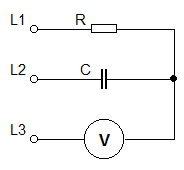
\includegraphics[scale=0.8]{schema-v.png}
\caption{Stanovení sledu fází voltmetrem}
\end{figure}

\section{Naměřené a vypočítané hodnoty}
Při měření nelze přesně určit, která fáze je která, ale můžeme přesně určit jejich sled například pomocí zkoušečky ZN1. Pokud jsou totiž fáze ve správném sledu, napětí je větší než zápalné napětí doutnavky ve zkoušečce a zkoušečka (doutnavka) svítí. Při nesprávném sledu fází se doutnavka přirozeně nerozsvítí. Se touto znalostí bylo změřeno, že jsou ve fázi následující kombinace fází: L1-L2, L2-L3, L3-L1. Jedině v těchto případech doutnavka svítila. V protifázi jsou kombinace: L3-L2, L2-L1, L1-L3. V tomto případě doutnavka nesvítila.

Pokud chceme stanovit sled fází pomocí voltmetru, musíme změřit napětí na jednotlivých fázích. Byla provedena dvě meření první pro připojení R na L1 a C na L2, druhé pro připojení R na L2 a C na L1:
\begin{table}[H]
\center
\caption{Naměřená napětí pomocí voltmetru}
\begin{tabular}{|c|c|c|c|}
\hline 
Měření & $U_V [V]$ & $U_R [V]$ & $U_C [V]$ \\ 
\hline 
1) měření & 167 & 95 & 80 \\ 
\hline 
2) měření & 47,5 & 95 & 80 \\ 
\hline 
\end{tabular} 
\end{table}
\begin{figure}[H]
\center
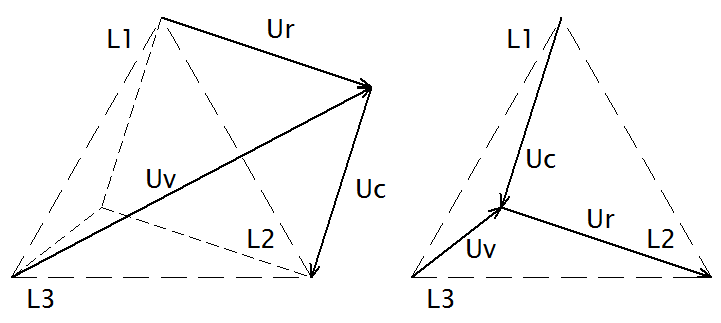
\includegraphics[scale=0.6]{fazor.png}
\caption{Fázorové diagramy}
\end{figure}
Fázorové diagramy jsou vůči sobě v měřítku, tzn. lze snadno poznat, že geometricky odpovídá první měření, tedy levý fázorový diagram. To odpovídá i předpokladu, že podle schématu by měla být velikost vektoru napětí $U_V$ větší, než ostatní vektory napětí, což tento diagram dokazuje.

Přístrojem USLO nebylo měření prováděno, jelikož má na měření v těchto laboratorních podmínkách nevhodné koncovky a nelze na trasformátor upnout.

\section{Závěr}
Při tomto měření jsme si ověřili správný sled fází střídavého zdroje. Při ověřování jsme použili zkoušečku ZN1. V dalším bodu měření jsme stanovili správný sled fází pomocí voltmetru na RC zátěži a následovně  změřili pro správný a nesprávný sled fází všechna jejich napětí. Měření pomocí voltmetru jsme prováděli na 3F zdroji 3x120V. Měření pomocí zkoušečky jsme prováděli na zdroji 3x400V.

\section{Přístroje}
\begin{itemize}
\item Voltmetr UNI21, evid. 13838
\item Transformátor 3x120V/3A, evid. 149559
\item Transformátor 3x400V/6A
\end{itemize}

\end{document}
